\section{Submission State Machine}\label{ch:6}

\subsection{Status vocabulary}

Statuses are defined once in \texttt{statuses.\allowbreak{}py} and never written as bare strings: \texttt{Not
Submitted}, \texttt{Processing}, \texttt{Submitted to OSG}, \texttt{Completed}, \texttt{Submission scripts
generated}, and the terminal \texttt{Failed to Read Directory}. Comparisons import these constants.

\subsection{State-transition diagram}

\begin{figure}[htbp]
  \centering
  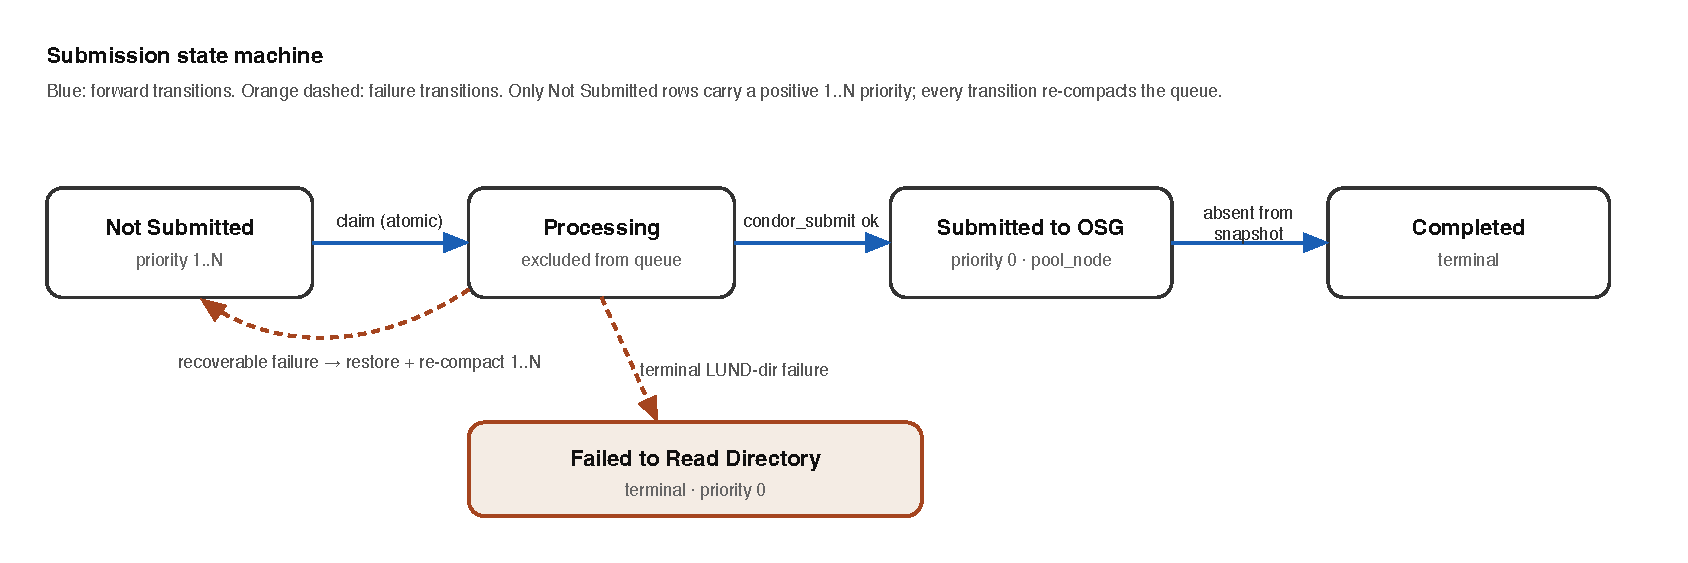
\includegraphics[width=\textwidth]{figures/fig2_state_machine}
  \caption{Submission state machine. States are defined once in \texttt{statuses.py}; the claim (Not Submitted
  $\rightarrow$ Processing) is an atomic status change, so at most one engine invocation submits a row. Only
  Not Submitted rows carry a positive $1..N$ priority, and every transition re-compacts the queue.}
  \label{fig:statemachine}
\end{figure}

\subsection{Priority values per state}

\texttt{Not Submitted} rows hold a unique pending position \texttt{1.\allowbreak{}.\allowbreak{}N}.
\texttt{Processing} rows are excluded from the pending queue. \texttt{Submitted to OSG} and \texttt{Failed to
Read Directory} rows hold priority \texttt{0} (they are out of the queue). The mapping is summarized in the
transitions table of Chapter 6.7 and the README.

\subsection{Atomic claim and race avoidance}

\texttt{mark\_\allowbreak{}submission\_\allowbreak{}processing()} performs the claim as an atomic status change
from \texttt{Not Submitted} to \texttt{Processing}. If another engine invocation claimed the row first, the
update affects no rows and the caller exits without submitting. This is what makes it safe to run the engine
concurrently or with an explicit \texttt{-\allowbreak{}b ID} target.

\subsection{Terminal and recoverable failure handling}

If \texttt{condor\_\allowbreak{}submit} is not reached, the row is restored to \texttt{Not Submitted} and the
queue re-compacted --- the request simply returns to the pending queue. A type-2 submission whose LUND
directory cannot be read is a terminal failure: the row receives \texttt{Failed to Read Directory} and priority
0, and is not retried.

\subsection{Invariants and idempotency}

Two invariants hold across all transitions: the pending queue is always contiguous
\texttt{1.\allowbreak{}.\allowbreak{}N}, and a row can be claimed by at most one engine invocation. Together
they make the engine idempotent --- re-running it never double-submits a request and never corrupts the queue.
